\section*{BT ÔN TẬP HỆ THỨC LƯỢNG SỐ 2}
% \subsection*{Đề số 2}
\setcounter{ex}{0}\setcounter{ex}{0}
\Opensolutionfile{ans}[ans/ans-KT-302]
% \noindent\textbf{I. PHẦN TRẮC NGHIỆM}
\begin{ex} 
	Cho $x\in(90^\circ;180^\circ)$. Phát biểu nào sau đây sai?
	\choice
	{$\tan x<0$}
	{$\cot x<0$}
	{$\sin x>0$}
	{\True $\cos x>0$}
	\loigiai{
		Do $x\in\left( 90^\circ;180^\circ\right)$ nên $\heva{&\sin x>0\\&\cos x<0\\&\tan x<0\\&\cot x<0.}$ }
\end{ex}
\begin{ex}
	Cho $\cos\alpha=-\dfrac{2}{5}$, với $90^\circ<\alpha<180^\circ$. Khi đó, $\tan\alpha$ bằng
	\choice
	{$\dfrac{\sqrt{21}}{5}$}
	{\True $-\dfrac{\sqrt{21}}{2}$}
	{$-\dfrac{\sqrt{21}}{5}$}
	{$\dfrac{\sqrt{21}}{2}$}
	\loigiai{
		Vì $90^\circ<\alpha<180^\circ$ nên $\sin\alpha>0$. Do đó, $\sin\alpha=\sqrt{1-\cos^2\alpha}=\dfrac{\sqrt{21}}{5}$.\\
		Suy ra $\tan\alpha=-\dfrac{\sqrt{21}}{2}$.
	}
\end{ex}
\begin{ex}
	Tính giá trị của $\cot150^\circ$.
	\choice
	{$\cot150^\circ=\sqrt{3}$}
	{\True $\cot150^\circ=-\sqrt{3}$}
	{$\cot150^\circ=\dfrac{\sqrt{3}}{3}$}
	{$\cot150^\circ=-\dfrac{\sqrt{3}}{3}$}
	\loigiai{
		Ta có $\cot150^\circ=-\cot30^\circ=-\sqrt{3}$.
	}
\end{ex}
\begin{ex}
	Khẳng định nào sau đây đúng?
	\choice
	{$\sin 90^\circ<\sin 100^\circ$}
	{\True $\cos 95^\circ>\cos 100^\circ$}
	{$\tan 85^\circ<\tan 125^\circ$}
	{$\cos 145^\circ>\cos 125^\circ$}
	\loigiai
	{Trong khoảng từ $90^\circ$ đến $180^\circ$, khi giá trị của góc tăng thì:\\
		- Giá trị $\sin$ tương ứng của góc đó giảm.\\
		- Giá trị $\cos$ tương ứng của góc đó giảm}
\end{ex}
\begin{ex}
	Phát biểu nào sau đây là đúng?
	\choice
	{\True $\sin78^\circ>0$}
	{$\cos 140^\circ>0$}
	{$\tan75^\circ<0$}
	{ $\cot20^\circ<0$}
	\loigiai{
		Ta có $\sin78^\circ>0$; $\cos 140^\circ<0$; $\tan75^\circ>0$; $\cot20^\circ>0$.
	}   
\end{ex}
\begin{ex} 
	Khi $x$ thuộc khoảng nào sau đây thì $P=\tan x\cdot\sin x$ nhận giá trị dương?
	\choice
	{$\left(0;180^\circ\right)$}
	{$\left(90^\circ;180^\circ\right)$}
	{$\left(45^\circ;145^\circ\right)$}
	{\True $\left(0;90^\circ\right)$}
	\loigiai{
		Ta có $P=\tan x\cdot\sin x=\dfrac{\sin^2 x}{\cos x}$. Do đó $P>0\Leftrightarrow \cos x>0$.
		
		\noindent Trong các khoảng đề cho thì ta thấy khi $x\in\left(0^\circ;90^\circ\right)$ thì $\cos x>0$ do đó $P>0$.
	}   
\end{ex}
\begin{ex}
	Trong các khẳng định sau đây, khẳng định nào \textbf{sai?}
	\choice
	{$\cos 45^\circ=\sin 45^\circ$}
	{$\cos 45^\circ=\sin {135^\circ}$}
	{$\cos 30^\circ=\sin 120^\circ$}
	{\True $\sin 60^\circ=\cos 120^\circ$}
	\loigiai
	{Bằng cách tra bảng giá trị lượng giác của các góc đặc biệt hay dùng MTCT ta được $\heva{& \cos 120^\circ=-\dfrac{1}{2} \\ 
			& \sin 60^\circ=\dfrac{\sqrt{3}}{2} \\ 
		}$.}
\end{ex}
\begin{ex}
	Giá trị của $\tan180^\circ$ bằng
	\choice
	{$1$}
	{\True $0$}
	{$-1$}
	{Không xác định}
	\loigiai{
		$\tan180^\circ=0$.
	}
\end{ex}
\begin{ex}
	Cho biết $\tan\alpha=\dfrac{1}{2}$. Tính $\cot\alpha$
	\choice
	{\True $\cot\alpha=2$}
	{$\cot\alpha=\dfrac{1}{4}$}
	{$\cot\alpha=\dfrac{1}{2}$}
	{$\cot\alpha=\sqrt{2}$}
	\loigiai{
		Ta có $\cot\alpha=\dfrac{1}{\tan\alpha}=2$.
	}
\end{ex}
\begin{ex}
	Giá trị lượng giác nào sau đây là số dương?
	\choice
	{$\tan 150^\circ$}
	{$\cos 130^\circ$}
	{$\tan 120^\circ$}
	{\True $\sin 170^\circ$}
	\loigiai{
		Dễ thấy rằng $\tan 150^\circ<0$, $\cos 130^\circ<0$, $\tan 120^\circ<0$ và $\sin 170^\circ>0$.} 
\end{ex} 
\begin{ex}
	Tìm mệnh đề đúng trong các mệnh đề sau.
	\choice
	{$\sin 60^\circ=\dfrac{\sqrt{2}}{2}$}
	{$\tan 30^\circ=\sqrt{3}$}
	{$\cot 90^\circ=1$}
	{\True $\sin 135^\circ=\dfrac{\sqrt{2}}{2}$}
	\loigiai{
		Mệnh đề đúng là $\sin 135^\circ=\sin 45^\circ=\dfrac{\sqrt{2}}{2}$.
}
\end{ex}
\begin{ex}
	Tìm mệnh đề đúng trong các mệnh đề sau
	\choice
	{\True $\sin\alpha=\sin(180^\circ-\alpha)$}
	{$\cos\alpha=\cos(180^\circ-\alpha)$}
	{$\tan\alpha=\tan(180^\circ-\alpha)$}
	{$\cot\alpha=\cot(180^\circ-\alpha)$}
	\loigiai{
		Mệnh đề đúng là $\sin\alpha=\sin(180^\circ-\alpha)$.
}
\end{ex}
\begin{ex}
	Biết $\sin\alpha=\dfrac{1}{3}$. Tính $P=\cos^2\alpha+3\tan^2\alpha$.
	\choice
	{\True $\dfrac{91}{72}$}
	{$\dfrac{5}{6}$}
	{$\dfrac{8}{9}$}
	{$\dfrac{67}{72}$}
	\loigiai{
		Ta có 
		\begin{eqnarray*}
		&P&=\cos^2\alpha+3\tan^2\alpha\\
		&&=1-\sin^2\alpha+3\dfrac{\sin^2\alpha}{\cos^2\alpha}\\
		&&=1-\sin^2\alpha+3\dfrac{\sin^2\alpha}{1-\sin^2\alpha}\\
		&&=1-\left(\dfrac{1}{3}\right)^2+3\dfrac{\left( \frac{1}{3}\right)^2}{1-\left(\frac{1}{3}\right)^2}\\
		&&=\dfrac{91}{72}.
		\end{eqnarray*}
}
\end{ex}
\begin{ex}
	Cho góc $\alpha$ sao cho $0^\circ\leq\alpha\leq 180^\circ$, khẳng định nào dưới đây là đúng?
	\choice
	{$\sin\alpha+\cos\alpha=1$}
	{$\cos\alpha>0$}	
	{\True $\sin^2\alpha+\cos^2\alpha=1$}
	{$\tan\alpha>0$} 
	\loigiai{
		Khẳng định đúng là $\sin^2\alpha+\cos^2\alpha=1$.
}
\end{ex}
\begin{ex}
	Trong mặt phẳng tọa độ $Oxy$, lấy điểm $M$ trên nửa đường tròn đơn vị sao cho $\widehat{xOM}=135^\circ$. Tìm hoành độ của điểm $M$.
	\choice
	{\True $-\dfrac{\sqrt{2}}{2}$}
	{$\dfrac{\sqrt{2}}{2}$}
	{$-\dfrac{\sqrt{3}}{2}$}
	{$-\dfrac{1}{2}$}
	\loigiai{
		Ta có $x_M=\cos 135^\circ=-\dfrac{\sqrt{2}}{2}$.
}
\end{ex}
\begin{ex}
	Tính giá trị của biểu thức $y=\cos^2 115^\circ+\cos^2 35^\circ+\sin^2 145^\circ +\sin^2 65^\circ$.
	\choice
	{$1$}
	{$3$}
	{$4$}
	{\True $2$}
	\loigiai{
		Do các cặp góc $65^\circ$ và $115^\circ$; $145^\circ$ và $35^\circ$ là các góc bù nhau nên $\cos 115^\circ=-\cos 65^\circ$; $\cos 35^\circ=-\cos 145^\circ$.\\
		Suy ra $y=\left(\cos^2 65^\circ+\sin^2 65^\circ \right)+\left(\cos^2 145^\circ+\sin^2 145^\circ \right) =1+1=2$.
	}
\end{ex}
\begin{ex}
	Khẳng định nào sau đây \textbf{đúng}?
	\choice
	{$\sin 90^\circ <\sin 100^\circ $}
	{\True $\cos 95^\circ >\cos 100^\circ $}
	{$\tan 85^\circ <\tan 125^\circ $}
	{$\cos 145^\circ >\cos 125^\circ $}
	\loigiai
	{Trong khoảng từ $90^\circ $ đến $180^\circ $, khi giá trị của góc tăng thì:\\
		- Giá trị $\sin$ tương ứng của góc đó giảm.\\
		- Giá trị $\cos$ tương ứng của góc đó giảm}
\end{ex}
\begin{ex}
	Tính diện tích $S$ của tam giác $ABC$ có độ dài ba cạnh là $5$ cm, $7$ cm và $8$ cm.
	\choice
	{$S=140$ cm$^2$}
	{\True $S=10\sqrt{3}$ cm$^2$}
	{$S=20$ cm$^2$}
	{$S=60\sqrt{13}$ cm$^2$}
	\loigiai{
		Ta có nữa chu vi của $\triangle ABC$ là $p=\dfrac{5+7+8}{2}=10$ cm.\\
		Diện tích $\triangle ABC$ là $S=\sqrt{10(10-5)(10-7)(10-8)}=10\sqrt{3}$ cm$^2$.
}
\end{ex}
\begin{ex}
	Cho tam giác $ABC$ có $AC=5$ cm, $BC=8$ cm và diện tích $S=10\sqrt{3}$ cm$^2$. Tìm số đo góc $ACB$.
	\choice
	{\True $\widehat{ACB}=60^{\circ}$}
	{$\widehat{ACB}=45^{\circ}$}
	{$\widehat{ACB}=90^{\circ}$}
	{$\widehat{ACB}=30^{\circ}$}
	\loigiai{
		Ta có\\
		 $S_{\triangle ABC}=\dfrac{1}{2}AC\cdot BC\cdot\sin\widehat{ACB}\Rightarrow\sin\widehat{ACB}=\dfrac{2S_{\triangle ABC}}{AC\cdot BC}=\dfrac{2\cdot 10\sqrt{3}}{5\cdot 8}=\dfrac{\sqrt{3}}{2}\Rightarrow\widehat{ACB}=60^\circ$.
}
\end{ex}
\begin{ex}
	Cho tam giác $ABC$ bất kì có $AB=c$, $BC=a$, $AC=b$ và $R$ là bán kính đường tròn ngoại tiếp tam giác $ABC$. Đẳng thức nào sau đây là đẳng thức đúng?
	\choice
	{$\dfrac{a}{\sin A}=\dfrac{b}{\sin B}=\dfrac{c}{\sin C}=R$}
	{\True $\dfrac{a}{\sin A}=\dfrac{b}{\sin B}=\dfrac{c}{\sin C}=2R$}
	{$\dfrac{a}{\sin A}=\dfrac{b}{\sin B}=\dfrac{c}{\sin C}=\dfrac{1}{2R}$}
	{$\dfrac{a}{\sin A}=\dfrac{b}{\sin B}=\dfrac{c}{\sin C}=\dfrac{1}{R}$}
	\loigiai{
		Đẳng thức đúng là $\dfrac{a}{\sin A}=\dfrac{b}{\sin B}=\dfrac{c}{\sin C}=2R$.
}
\end{ex}
\begin{ex}
	Cho tam giác $ABC$ có $\widehat{B}=45^\circ$, $\widehat{C}=75^\circ$ và cạnh $BC=5$. Bán kính đường tròn ngoại tiếp tam giác $ABC$ là
	\choice
	{$5$}
	{$\dfrac{5}{2}$}
	{\True $\dfrac{5 \sqrt{3}}{3}$}
	{$\dfrac{5 \sqrt{3}}{2}$}
	\loigiai{
		Ta có $\widehat{A}=180^\circ-\widehat{B}-\widehat{C}=180^\circ-45^\circ-75^\circ=60^\circ$.\\
		Theo định lí $\sin$ trong tam giác ta có $\dfrac{BC}{\sin A}=2R\Rightarrow R=\dfrac{BC}{2\sin A}=\dfrac{5}{2\cdot\sin 60^\circ}=\dfrac{5\sqrt{3}}{3}$.
}
\end{ex}
\begin{ex}
	Cho tam giác $ABC$ có các cạnh $BC=a=6\ \mathrm{cm},\ AC=b=7\ \mathrm{cm},\ AB=c=5\ \mathrm{cm}$. Tính $\cos B$.
	\choice
	{$\cos B=\dfrac{5}{7}$}
	{$\cos B=\dfrac{19}{35}$}
	{$\cos B=\dfrac{1}{15}$}
	{\True $\cos B=\dfrac{1}{5}$}
	\loigiai{
		Ta có: $$\cos B=\dfrac{a^2+c^2-b^2}{2ac}=\dfrac{6^2+5^2-7^2}{2\cdot 6\cdot 5}=\dfrac{1}{5}.$$
	}
\end{ex}
\begin{ex}
	Cho tam giác $ABC$ có $BC=a$, $CA=b$, $AB=c$. Chọn đẳng thức \textbf{sai}.
	\choice
	{$b^2=a^2+c^2-2ac\cos B$}
	{$a^2=b^2+c^2-2bc\cos A$}
	{\True $c^2=b^2+a^2+2ab\cos C$}
	{$c^2=b^2+a^2-2ab\cos C$}
	\loigiai{
		Theo định lý côsin trong tam giác $ABC$, ta có $c^2=b^2+a^2-2ab\cos C$.}
\end{ex}
\begin{ex}
	Trong tam giác $ABC$ có
	\choice
	{$m_a=\dfrac{b+c}{2}$}
	{$m_a>\dfrac{b+c}{2}$}
	{\True $m_a<\dfrac{b+c}{2}$}
	{$m_a=b+c$}
	\loigiai{
		Ta có $\left\{\begin{aligned}
		&m_a^2=\dfrac{2(b^2+c^2)-a^2}{4}\\
		&a>|b-c|.\\
		\end{aligned}\right. $ \\
		Suy ra $m_a^2<\dfrac{2(b^2+c^2)-(b-c)^2}{4}=\dfrac{b^2+c^2+2bc}{4}=\dfrac{(b+c)^2}{4}$.\\
		Hay $m_a<\dfrac{b+c}{2}$.}
\end{ex}
\begin{ex}
	Cho tam giác $ABC$ có góc $\widehat{B}=60^{\circ}, \widehat{C}=45^{\circ}$, $AB=9$. Độ dài cạnh $AC$ là
	\choice
	{$\dfrac{6\sqrt{6}}{2}$}
	{$3\sqrt{6}$}
	{\True $\dfrac{9\sqrt{6}}{2}$}
	{$\dfrac{4\sqrt{6}}{3}$}
	\loigiai{
		Áp dụng định lí sin ta có 
		\[ \dfrac{AC}{\sin B}=\dfrac{AB}{\sin C} \Rightarrow AC=\dfrac{AB\cdot\sin B}{\sin C}=\dfrac{9\cdot \sin 60^\circ}{\sin 45^\circ}=\dfrac{9\sqrt{6}}{2}.\]
	}
\end{ex}
\begin{ex}
	\immini{
		Trên nóc một tòa nhà có một cột ăng-ten cao $6$ m. Từ vị trí quan sát $A$ cao $3$ m so với mặt đất, có thể nhìn thấy đỉnh $B$ và chân $C$ của cột ăng-ten dưới góc $55^{\circ}$ và $45^{\circ}$ so với phương ngang. Chiều cao của tòa nhà gần nhất với số nào dưới đây?
		\choice
		{\True $17$ m}
		{$17{,}1$ m}
		{$18{,}1$ m}
		{$18$ m}
	}
	{
		\begin{tikzpicture}[scale=1, font=\footnotesize, line join=round, line cap=round,>=stealth]
		\path 
		(0,0) coordinate (A)
		(4,3) coordinate (C)
		(4,4.2) coordinate (B) 
		(0,-1) coordinate (A') 
		(4,0) coordinate (H) 
		;
		\draw[fill=gray!30] (B)--(C) (C)--(6,3)--(6,-1)--(4,-1)--(C) (-0.5,-1)--(6.6,-1);
		\draw  (C)--(6,3)--(6,-1)--(4,-1)--(C);
		\foreach \i in {2,3,4,5}
		\draw[fill=cyan!40] ({4+1/3},{-1+(2/3)*(\i-1)})--({4+1/3},{-1+(2/3)*(\i-1)+0.5})--({4+2/3},{-1+(2/3)*(\i-1)+0.5})--({4+2/3},{-1+(2/3)*(\i-1)})--cycle 
		({5+1/3},{-1+(2/3)*(\i-1)})--({5+1/3},{-1+(2/3)*(\i-1)+0.5})--({5+2/3},{-1+(2/3)*(\i-1)+0.5})--({5+2/3},{-1+(2/3)*(\i-1)})--cycle;
		\draw[dashed](A)--(B)  (A)--(C) (A)--(H); 
		\draw [<->](A)--(A');
		\draw ($(B)!0.5!(C)$) node[right]{$6\mathrm{~m}$} ($(A)!0.5!(A')$) node[left]{$3 \mathrm{~m}$} ;
		\draw pic["$55^{\circ}$", draw=black, angle eccentricity=1.2, angle radius=1.4cm]{angle=H--A--B};
		\draw pic["$45^{\circ}$", draw=black,double, angle eccentricity=1.5, angle radius=0.7cm]{angle=H--A--C};
		\foreach \x/\g in {A/180,B/90,C/140} 
		\fill[black] (\x) circle (1pt)+(\g:3mm) node {$\x$};
		\clip (-0.5,{-1-0.25}) rectangle (6.6,-1) ;
		\draw[fill=gray!30] (-0.5,-1)--(6.6,-1)--(6.6,{-1-0.25})--(-0.5,{-1-0.25})--cycle;
		\foreach \i in {1,2,...,35}
		\draw ({-0.5+0.2*(\i)},-1)--($({-0.5+0.2*(\i)},-1)+(-120:0.3)$) ;
		\end{tikzpicture}
	}
	\loigiai{
		\immini{
			Gọi $H$ là hình chiếu vuông góc của $A$ trên $BC$; $M,N$ là hình chiếu vuông góc của $A$ và $B$ trên mặt đất. \\
			Đặt $AH=x$ ta có $BH = x\tan 55^\circ$ và $CH = x\tan 45^\circ$.\\
			Theo giả thiết 
			\[ BC=6 \Leftrightarrow x(\tan 55^\circ - \tan 45^\circ) = 6 \Leftrightarrow x = \dfrac{6}{\tan 55^\circ - \tan 45^\circ}.\]
			Chiều cao tòa nhà là 
			\[ CN=HN + CH = 3+ \dfrac{6\tan 45^\circ}{\tan 55^\circ - \tan 45^\circ} \approx 17 \mathrm{~m}. \]
		}
		{
			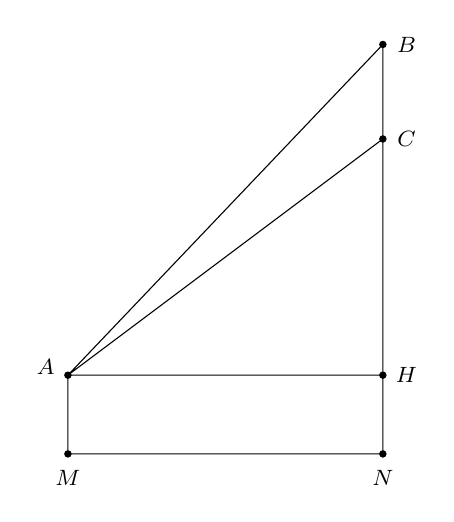
\begin{tikzpicture}[scale=1,font=\footnotesize, line join=round, line cap=round, >=stealth]
			\path 
			(0,0) coordinate (A)
			(4,3) coordinate (C)
			(4,4.2) coordinate (B) 
			(0,-1) coordinate (M) 
			(4,-1) coordinate (N)
			(4,0) coordinate (H) 
			;
			\draw (B)--(A)--(C) (H)--(A)--(M)--(N)--(B);
			\foreach \x/\y in {B/0,C/0,A/160,H/0,M/-90,N/-90}
			\draw[fill=black] (\x) circle (0.04cm) + (\y:0.3cm) node {$\x$};
			\end{tikzpicture}
		}
	}
\end{ex}
\begin{ex}
	Cho tam giác $ABC$ có $BC=5$cm, góc $\widehat{BAC}=30^\circ$. Bán kính đường tròn ngoại tiếp tam giác $ABC$ bằng
	\choice
	{\True $5$ cm}
	{$10$ cm}
	{$5\sqrt{3}$ cm}
	{$\dfrac{5\sqrt{3}}{3}$ cm}
	\loigiai{Bán kính đường tròn ngoại tiếp tam giác $ABC$ là $R=\dfrac{BC}{2\sin\widehat{BAC}}=\dfrac{5}{2\sin30^\circ}=5$ cm.}
\end{ex}
\begin{ex}
	Cho tam giác $ABC$ có $AB=\sqrt{2}$, $\widehat{B}=60^{\circ}$, $\widehat{C}=45^{\circ}$. Tính độ dài đoạn $AC$.
	\choice
	{\True $AC=\sqrt{3}$}
	{$AC=\dfrac{\sqrt{3}}{2}$}
	{$AC=3$}
	{$AC=\dfrac{\sqrt{3}}{3}$}
	\loigiai{
		\immini{
			Ta có: $\widehat{A}=180^{\circ}-\left(\widehat{B}+\widehat{C}\right)=180^{\circ}-\left(60^{\circ}+45^{\circ}\right)=75^{\circ}$.\\
			Theo định lý Sin ta có: $\dfrac{AC}{\sin B}=\dfrac{AB}{\sin C}$.\\
			Suy ra $AC=\dfrac{AB\cdot\sin B}{\sin C}=\dfrac{\sqrt{2}\cdot\sin 60^{\circ}}{\sin 45^{\circ}}=\sqrt{3}.$}
		{\vspace{-0.5cm}
			\begin{tikzpicture}[scale=0.8,>=stealth, font=\footnotesize, line join=round, line cap=round]
			\path
			(0,0) coordinate (A) node [below]{$A$}
			(1,3) coordinate (B) node [above]{$B$}
			(3,0) coordinate (C) node [below]{$C$}
			;
			\draw (A)--(B)--(C)--cycle;
			\foreach \x in {A,B,C} \draw[fill=black] (\x) circle (1pt);
			\node at ($(C)+(160:20pt)$) {$45^\circ$};
			\node at ($(B)+(-80:20pt)$) {$60^\circ$};
			\end{tikzpicture}}}
\end{ex}
\begin{ex}
	Cho tam giác $ABC$ có $a=13$ m, $b= 14$ m, $c=15$ m. Tính diện tích $S$ của tam giác $ABC$.
	\choice
	{\True $S= 84$ m$^2$}
	{$S= 90$ m$^2$}
	{$S= 76$ m$^2$}
	{$S= 80$ m$^2$}
	\loigiai{
		Ta có: $p=\dfrac{a+b+c}{2} =21$ và $$S=\sqrt{p(p-a)(p-b)(p-c)}=\sqrt{21(21-13)(21-14)(21-15)} =84\text{ m}^2.$$ 
	}
\end{ex}
\begin{ex}
	Một hình bình hành có độ dài hai cạnh kề lần lượt là $16$ cm và $24$ cm. Một đường chéo  có độ dài là $32$ cm. Tính góc đối diện với đường chéo đó.
	\choice
	{$101{,}3^\circ$}
	{$107{,}3^\circ$}
	{$100{,}7^\circ$}
	{\True $104{,}5^\circ$}
	\loigiai{
		\immini{
			Gọi góc đối diện với đường chéo là $\alpha$. \\
			Áp đụng định lí cô sin ta có
			\[
			\cos \alpha = \dfrac{24^2+16^2-32^2}{2 \cdot 24 \cdot 16} = -\dfrac{1}{4} \Rightarrow \alpha \approx 104{,}5^\circ.
			\]
		}
		{
			\begin{tikzpicture}[scale=1, font=\footnotesize, line join=round, line cap=round,>=stealth]
			\path
			(0,0) coordinate (A)
			(1,2) coordinate (B)
			(4,2) coordinate (C)
			(3,0) coordinate (D)
			;
			\draw (A)--(B)--(C)--(D)--(A)--(C);  
			\draw ($(A)!0.5!(D)$) node[below]{$24\mathrm{cm}$} ($(D)!0.5!(C)$) node[right]{$16\mathrm{cm}$}  ($(A)!0.5!(C)$) node[above=2pt]{$32\mathrm{cm}$};
			\foreach \x/\g in {A/-120,B/-60,C/90,D/90} 
			\fill[black] (\x) circle (1pt)+(\g:3mm) node {$ $};
			\end{tikzpicture}
		}
	}
\end{ex}
\begin{ex}
	Cho tam giác $ABC$ có $AB=5$, $AC=4$, trung tuyến $BM=\sqrt{33}$. Tính diện tích $S$ của tam giác $ABC$.
	\choice
	{$S=3\sqrt{6}$}
	{\True $S=4\sqrt{6}$}
	{$S=2\sqrt{13}$}
	{$S=24\sqrt{33}$}
	\loigiai{Do $M$ là trung điểm của $AC$ nên $AM=\dfrac{1}{2}AC=2$. Xét tam giác $AMB$ ta có
		$$\cos\widehat{BAM}=\dfrac{AB^2+AM^2-BM^2}{2\cdot AB\cdot AM}=\dfrac{25+4-33}{2\cdot 5\cdot 2}=-\dfrac{1}{5}.$$
		Có $\sin\widehat{BAM}=\sqrt{1-\cos^2\widehat{BAM}}=\dfrac{2\sqrt{6}}{5}$, suy ra diện tích tam giác $ABC$ là
		$$S_{ABC}=\dfrac{1}{2}\cdot AB\cdot AC\cdot \sin\widehat{BAM}=\dfrac{1}{2}\cdot 5\cdot 4\cdot \dfrac{2\sqrt{6}}{5}=4\sqrt{6}.$$
	}
\end{ex}
\begin{ex}
	Tam giác $ABC$ có $AB=9$ cm, $AC=12$ cm và $BC=15$ cm. Khi đó đường trung tuyến $AM$ của tam giác có độ dài là
	\choice
	{$8$ cm}
	{$10$ cm}
	{$9$ cm}
	{\True $7{,}5$ cm}
	\loigiai{
		Ta có\\
		$$AM^2=\dfrac{AB^2+AC^2}{2}-\dfrac{BC^2}{4}=\dfrac{225}{4}\Leftrightarrow AM=7{,}5.$$
	}
\end{ex}
\begin{ex}
	Cho tam giác $ABC$ có $\widehat{B}=135^\circ$. Khẳng định nào sau đây là đúng?
	\choice
	{$R=\dfrac{a}{\sin A}$}
	{\True $R=\dfrac{\sqrt{2}}{2}b$}
	{$R=\dfrac{\sqrt{2}}{2}c$}
	{$R=\dfrac{\sqrt{2}}{2}a$}
	\loigiai{
		Ta có $\dfrac{b}{\sin B}=2R$. Suy ra $R=\dfrac{b}{2\sin B}=\dfrac{b}{2\cdot \sin 135^\circ}=\dfrac{\sqrt{2}}{2}b$.
	}
\end{ex}
\begin{ex}
	Cho tam giác $ABC$ có $a=\sqrt{6}$; $b=2$; $c=\sqrt{3}+1$. Tìm số đo của góc $A$.
	\choice
	{$45^{\circ}$}
	{\True $60^{\circ}$}
	{$30^{\circ}$}
	{$90^{\circ}$}
	\loigiai{
		$\cos A=\dfrac{b^2+c^2-a^2}{2bc}=\dfrac{2^2+\left(\sqrt{3}+1\right)^2-\left(\sqrt{6}\right)^2}{2 \cdot 2 \cdot \left(\sqrt{3}+1\right)}=\dfrac{1}{2} \Rightarrow \widehat{A}=60^{\circ}$.}
\end{ex}
\begin{ex}
	Cho tam giác $ABC$ có ba cạnh $a=13;b=14;c=15$. Bán kính của đường tròn ngoại tiếp tam giác $ABC$ bằng
	\choice
	{$4$}
	{$84$}
	{\True $\dfrac{65}{8}$}
	{$14$}
	\loigiai{
		Ta có $p=\dfrac{a+b+c}{2}=21$, $S=\sqrt{p(p-a)(p-b)(p-c)}=84$.\\
		Mà $S=\dfrac{abc}{4R} \Rightarrow R=\dfrac{abc}{4S}=\dfrac{65}{8}$.}
\end{ex}

\noindent\textbf{II. PHẦN TỰ LUẬN}
\begin{ex}
	Cho $\cos\alpha=-\dfrac{5}{9}$ và $90^\circ<\alpha<180^\circ$. Tính các giá trị lượng giác còn lại của góc $\alpha$.
	\loigiai{
		$\sin^2\alpha=1-\cos^2\alpha=1-\left(\dfrac59\right)=\dfrac{56}{81}$\\
		$\Rightarrow \sin\alpha=\sqrt{\dfrac{56}{81}}=\dfrac{2\sqrt{14}}{9}$ (vì $\sin\alpha\ge0,\forall \alpha$).\\
		Suy ra $\tan\alpha=\dfrac{\sin\alpha}{\cos\alpha}=-\dfrac{2\sqrt{14}}{5}$ và $\cot\alpha=\dfrac{1}{\tan\alpha}=-\dfrac{5\sqrt{14}}{28}$
	}
\end{ex}
% \begin{ex}
% 	Cho $\heva{&a=\sin x\\&b=\cos x\sin x\\&c=\cos x\cos y}$. Chứng minh rằng $a^2+b^2+c^2=1$.
% 	\loigiai{Ta có:
% 		\begin{align*}
% 		a^2+b^2+c^2 & =\sin^2x+\cos^2x(1-\cos^2y)+\cos^2x\cos^2y \\
% 		&=\sin^2x+\cos^2x-\cos^2x\cos^2y+\cos^2x\cos^2y\\
% 		&=1.
% 		\end{align*}
% 	}
% \end{ex}
\begin{ex}
	Cho tam giác $ABC$, chứng minh rằng	
		 $\cot A+\cot B+\cot C \geq \sqrt{3}$.
	\loigiai{
			Áp dụng định lí côsin và công thức $S=\dfrac{1}{2}bc\sin A$ ta có:\\
			$\cot A=\dfrac{\cos A}{\sin A}=\dfrac{b^{2}+c^{2}-a^{2}}{2 b c \sin A}=\dfrac{b^{2}+c^{2}-a^{2}}{4 S}$.\\
			Tương tự ta có $\cot B=\dfrac{c^{2}+a^{2}-b^{2}}{4 S}, \cot C=\dfrac{a^{2}+b^{2}-c^{2}}{4 S}$\\
			Suy ra $\cot A+\cot B+\cot C=\dfrac{b^{2}+c^{2}-a^{2}}{4 S}+\dfrac{c^{2}+a^{2}-b^{2}}{4 S}+\dfrac{a^{2}+b^{2}-c^{2}}{4 S}=\dfrac{a^{2}+b^{2}+c^{2}}{4 S}$.\\
			Theo bất đẳng thức Cauchy ta có $(p-a) (p-b) (p-c) \leq\left(\dfrac{3 p-a-b-c}{3}\right)^{3}=\left(\dfrac{p}{3}\right)^{3}$.\\
			Mặt khác $S=\sqrt{p(p-a)(p-b)(p-c)} \Rightarrow S \leq \sqrt{p\cdot \dfrac{p^{3}}{27}}=\dfrac{p^{2}}{3 \sqrt{3}}$.\\
			Ta có $p^{2}=\dfrac{\left(a+b+c^{2}\right) }{4} \leq \dfrac{3\left(a^{2}+b^{2}+c^{2}\right) }{4}$ suy ra $S \leq \dfrac{a^{2}+b^{2}+c^{2}}{4 \sqrt{3}}$.\\
			Do đó $\cot A+\cot B+\cot C \geq \dfrac{a^{2}+b^{2}+c^{2}}{4 \cdot \dfrac{a^{2}+b^{2}+c^{2}}{4 \sqrt{3}}}=\sqrt{3}$ .
	}
\end{ex}
\begin{ex}
	Cho tam giác $ABC$ có $AB=6$, $AC=8$ và $\widehat{A}=60^\circ$.
	\begin{enumerate}
		\item Tính diện tích tam giác $ABC$.
		\item Gọi $I$ là tâm đường tròn ngoại tiếp tam giác $ABC$. Tính diện tích tam giác $IBC$.
	\end{enumerate}
	\loigiai
	{
		\immini
		{
			\begin{enumerate}
				\item %Câu a
				Ta có 
				$$S=\dfrac{1}{2}AB\cdot AC\cdot \sin A=\dfrac{1}{2}\cdot 6\cdot 8\cdot \sin60^\circ=12\sqrt{3}.$$
				\item %Câu b
				Ta có $\widehat{BIC}=2\widehat{BAC}=120^\circ$\\
				Ta có
				$$BC=\sqrt{AB^2+AC^2-2AB\cdot AC\cdot \cos A}=\sqrt{6^2+8^2-2\cdot 6\cdot 8\cdot \dfrac{1}{2}}=2\sqrt{13}.$$ 
				Ta có 
				$$S=\dfrac{AB\cdot AC\cdot BC}{4R} \Rightarrow R=\dfrac{AB\cdot BC\cdot CA}{4S}=\dfrac{6\cdot 8\cdot 2\sqrt{13}}{4\cdot 12\sqrt{3}}=\dfrac{2\sqrt{39}}{3}$$
				Từ đó suy ra $IB=IC=R=\dfrac{2\sqrt{39}}{3}$.\\
				Vậy $S_{\triangle IBC}=\dfrac{1}{2}IB\cdot IC\cdot \sin \widehat{BIC}=\dfrac{1}{2}\cdot \dfrac{2\sqrt{39}}{3}\cdot \dfrac{2\sqrt{39}}{3}\cdot \sin 120^\circ\approx 7{,}5$.
			\end{enumerate}	
		}
		{
			\begin{tikzpicture}[scale=0.7, font=\footnotesize, line join=round, line cap=round,>=stealth]
			\def\canhBA{6};\def\canhAC{8};\def\gocBAC{60};
			%Định nghĩa điểm.
			\coordinate (A) at (0,0);
			\coordinate (B) at ($(A)+(\gocBAC:\canhBA)$);
			\coordinate (C) at ($(A)+(0:\canhAC)$);
			%Vẽ tam giác BAC.
			\draw (B)--(A)--(C)--cycle;
			%Hiển thị các điểm.
			\foreach \x/\y in {B/90, A/180, C/0}{\fill (\x) circle(1pt) ($(\x)+(\y:0.3cm)$) node{$\x$};}
			\end{tikzpicture}
		}
	}
\end{ex}
\Closesolutionfile{ans}
\Closesolutionfile{ansbook}
\indapan{10}{ans/ans-KT-302}